\documentclass{standalone}
\usepackage{tikz}
\usepackage{amsmath, amssymb}

\begin{document}
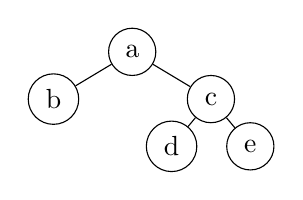
\begin{tikzpicture}[
    every node/.style={
      circle, draw, minimum width=6mm,
    }, 
    level/.style={
      sibling distance=20mm/#1,
      level distance=6mm
    }
    ]
  \node (n0) {a}
    child {
      node (n12) {b}
    }
    child {
      node (n11) {c}
      child {node (n21) {d}}
      child {node (n22) {e}}
    }
  ;
\end{tikzpicture}
\hspace{20mm} $\rightarrow$ \hspace{20mm}
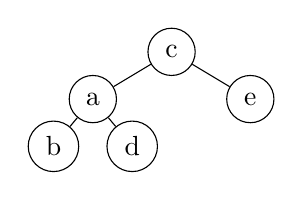
\begin{tikzpicture}[
    every node/.style={
      circle, draw, minimum width=6mm,
    }, 
    level/.style={
      sibling distance=20mm/#1,
      level distance=6mm
    }
    ]
  \node (n0) {c}
    child {
      node (n11) {a}
      child {node (n21) {b}}
      child {node (n22) {d}}
    }
    child {
      node (n12) {e}
    }
  ;
\end{tikzpicture}
\end{document}
